\section{Evaluation}\label{sec:eval}

\subsubsection{Setup.} One laptop core, pure Python; both arms run the same prover binary, one process per
execution, interleaved with rotating order (1 warm-up, 7 rounds), every proof verified after the timer stops. % no-evidence: protocol parameter
The metric is process CPU time of circuit build plus proving. Absolute times of a pure-Python toy mean nothing;
we report only ratios between the arms. Counts are read off the built circuits.

\begin{table}[t]
\centering
\caption{Counts for $n = 64$ values and $c = 8$ (padded height = next power of two of $\max(\text{rows}, 2^c)$).
R1CS constraints are a different unit and are listed for reference only.}\label{tab:counts}
% EVIDENCE E1 (whole table): results/counts/counts.log
\begin{tabular}{rrrrrrr}
\toprule
$k$ & R1CS constr. & bits rows & bits padded & lookup rows & lookups & lookup padded \\
\midrule
4  & 320  & 320  & 512  & 128 & 128 & 256 \\
8  & 576  & 576  & 1024 & 128 & 64  & 256 \\
12 & 832  & 832  & 1024 & 192 & 192 & 256 \\
16 & 1088 & 1088 & 2048 & 192 & 128 & 256 \\
32 & 2112 & 2112 & 4096 & 320 & 256 & 512 \\
64 & 4160 & 4160 & 8192 & 576 & 512 & 1024 \\
\bottomrule
\end{tabular}
\end{table}

\subsubsection{Rows.} \Cref{tab:counts} shows the trade-off. The bits arm grows with $k$ (4160 constraints\evid{E2}
in R1CS and 8192 rows\evid{E3} padded at $k = 64$), the lookup arm with $\lceil k/8 \rceil$ (1024 rows\evid{E4}), but
never below the 256 rows\evid{E8} of its table. The padded-height ratio is therefore 8$\times$\evid{E7} for
$16 \le k \le 63$ (and at $k = 64$), only 4$\times$\evid{E6} at $k = 8$ and $12$, and 2$\times$\evid{E5} at $k = 4$.

\begin{figure}[t]
\centering
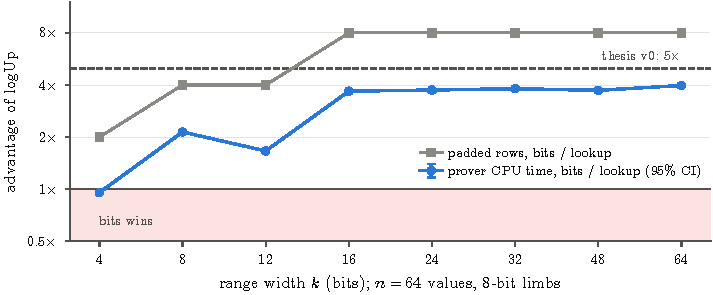
\includegraphics[width=\textwidth]{figs/fig_ratio_vs_k}
\caption{Advantage of the logUp encoding over running-sum bits ($n = 64$, $c = 8$), in padded rows and in toy
prover CPU time (median ratio, paired bootstrap 95\% confidence interval; CIs are narrower than the markers). % no-evidence: confidence level
Below $1\times$ the bit decomposition is faster.}\label{fig:ratio}
\end{figure}

\subsubsection{Prover time.} \Cref{fig:ratio} plots the measured ratios. For $16 \le k \le 48$ the lookup arm is
3.69$\times$\evid{E13}, 3.74$\times$\evid{E14}, 3.81$\times$\evid{E15} and 3.73$\times$\evid{E16}
faster (at $k = 16, 24, 32, 48$), and 3.98$\times$\evid{E17} at $k = 64$, which is outside the range-check domain; at $k = 8$ and $12$ it is 2.14$\times$\evid{E11} and 1.66$\times$\evid{E12}; at
$k = 4$ it is no faster, 0.96$\times$\evid{E10} (a re-run on the same machine gave parity, so we claim no more). The time ratio stays well below the row ratio because each lookup row
carries more committed columns (limb, multiplicities, helper columns) and more constraints in the zero-check;
an operation-count model of the prover predicts the dominant phases within a factor 1.5 at every point % no-evidence: tolerance (bench-protocol)
(\cref{app:checks}). The 5$\times$ of our initial thesis is not reached at any $k$. % no-evidence: the thesis' target

\subsubsection{Limb width and statement size.} The table is the price of the gain. At $k = 32$ and $n = 64$, 4-bit
limbs give 2.07$\times$\evid{E40} and 8-bit limbs 3.77$\times$\evid{E41}, while 16-bit limbs make the lookup arm
slower than bits, 0.04$\times$\evid{E42}, because the table alone fills $2^{16}$ rows. % no-evidence: 2^16 = table size for c = 16 (definition)
With only $n = 16$ values at $k = 16$ the two arms are even, 1.05$\times$\evid{E43}. These runs come from a
separate interleaved session with 5 rounds. % no-evidence: protocol parameter

\subsubsection{Limitations.} The toy has no polynomial commitment: the verifier reads the committed columns. With a
real commitment each committed column costs work proportional to the trace height, so the lookup arm pays more for
its extra columns and less for its smaller height than here; the ratios may move in either direction. We report
neither proof size nor verifier time, which are meaningless without a commitment scheme.
